\chapter{Rouge}
\label{ch:rouge}
\begin{quotation}
\textsl{You are a nameless traveller that has been compelled to search for something. An object, a person, or just a place. You don't know yet, but it's up to you to find out. You will travel through various caves, forests and towns to pursue the whims of your heart. Every time you seem to solve a problem, another one turns up. Always moving you towards some inevitable doom. Are you born for heroism, or will you die unloved and unknown? \\\\Choose your path, and see where the voices in your head take you.}
\end{quotation}
Rouge is a \rogue tile-based game that is created specifically for the demonstration of the \diage narrative generation system. Created within my own framework \textit{SilicaLib} created on top of the XNA game-framework created by Microsoft. Rouge is characterised by the fact that the world and the narrative is generated by the direct influence of the player. 
This section elaborates on how Rouge was made, what all the different algorithms are that were included, and gives definitive answers to my research questions from Chapter 1. 

\section{Mechanics}
The game mechanics in Rouge are fully implemented within the \diage attribute system. When ever actors interact with the world their attributes can effect the world according to their rules. Whenever they interact with other actors, these attributes will influence dialogue or cause either an antagonistic, friendly or neutral response in accordance to their moral alignment.

Actors move around the world in turns. When an entity gets the turn, its actions points are restored and he can use these to either move around the game world or attack an enemy. Attacking an other actor results in a damage step. This step subtracts the strength attribute of the attacker from the defence attribute and subtracts that outcome from the defenders health attribute. 

Normal interaction with other actors does not cost an action point and resolves in a simple conversation. The player asks the other actor for any information regarding his current quest. If the actor knows about it, it will give either helpful or hurtful information, depending upon his alignment attribute. The alignment resolution can also result in the actor refusing to answering the player's question if their alignments are to far apart from each other.  

\section{Cellular Automata}
The world within Rouge is procedurally generated by a cellular automaton. Celullar automata work by defining a regular grid of cells, each in any number of states. Using rules pertaining to the neighbours of each cell, that cell can change its state. For example; we define the states \textit{alive} and \textit{dead}. After that we define several rules:
\begin{enumerate}
	\item A cell goes into a \textit{dead} state when it has \underline{less} than 2 live neighbours.
	\item A cell goes into a \textit{dead} state when it has \underline{more} than 3 live neighbours.
	\item A cell goes into a \textit{alive} state when it has \underline{exactly} 3 neighbours.
\end{enumerate}
With these definitions set the grid could be populated with a random amount of cells in live state, assuming that the dead state is the default. Each step of the automaton will cycle through the rules, checking to see if the conditions of a rule is set. After all the cells have been checked the rules execute and changes the grid. The truly awesome thing that cellular automata bring with them, is the potential to emergent behaviour. With these three simple rules, we can generate moving shapes, and repeating patterns. The rules come from one of the most recognized cellular automata; \game{Conway's Game of Life}. Figure~\ref{fig:game_of_life} shows an example of the emergent behaviour that these simple rules generate. 

\begin{figure}[p]
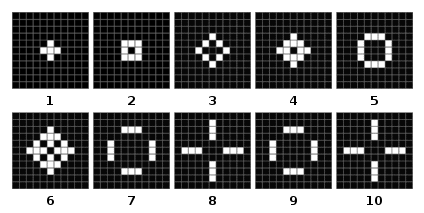
\includegraphics[width=.8\textwidth]{gameoflife}
\caption{An example of the Game of Life generation steps}\label{fig:game_of_life}
\end{figure}

During a step of this automaton, the algorithm walks through the game world and checks each tile for certain conditions pertaining to their neighbours. If these conditions are met, his state will be changed accordingly. The states a tile has in Rouge are a simple \textit{alive} or \textit{dead} state. When a tile has 5 or more live neighbours, the tile becomes alive themselves. However, when a tile has less than 2 live neighbours, the tile dies. The first rule ensures that tiles group together, and the other rule destroys any singular 'island' tiles.

\begin{algorithm}
	\KwIn{tilemap}
	\KwOut{new tilemap}
	let \textit{deadCells} and \textit{liveCells} be an empty collection of tiles\;
	\ForEach{tile in tilemap}{
		\uIf{tile.neighbours $\geq$ 5}{
			liveCells.push(tile)\;
		}\uElseIf{tile.neighbours $\leq$ 1}{
			deadCells.push(tile)\;
		}
	}
	\ForEach{tile in deadCells}{
		tile.alive = false\;
	}
	\ForEach{tile in liveCells}{
		tile.alive = true\;
	}
	\caption{Cellular Automation algorithm as used in Rouge}\label{alg:ca}
\end{algorithm}

\begin{figure}[p]
	\centering
	\begin{subfigure}[b]{0.3\textwidth}
		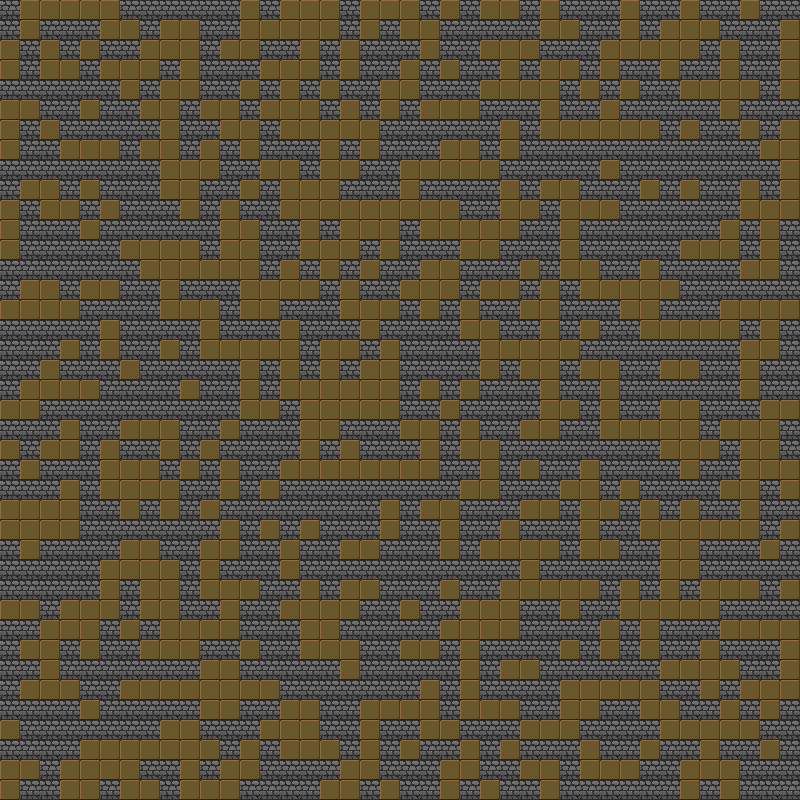
\includegraphics[width=\textwidth]{rouge/screenshot0}
		\caption{Initial map}
	\end{subfigure}	
	~
	\begin{subfigure}[b]{0.3\textwidth}
		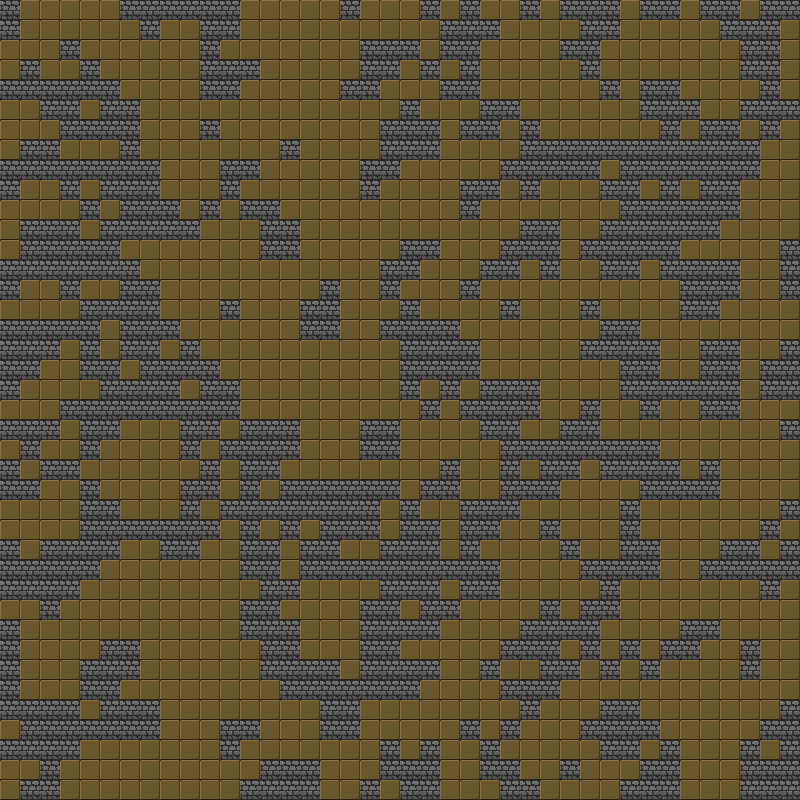
\includegraphics[width=\textwidth]{rouge/screenshot1}
		\caption{Step 1}
	\end{subfigure}	
	~
	\begin{subfigure}[b]{0.3\textwidth}
		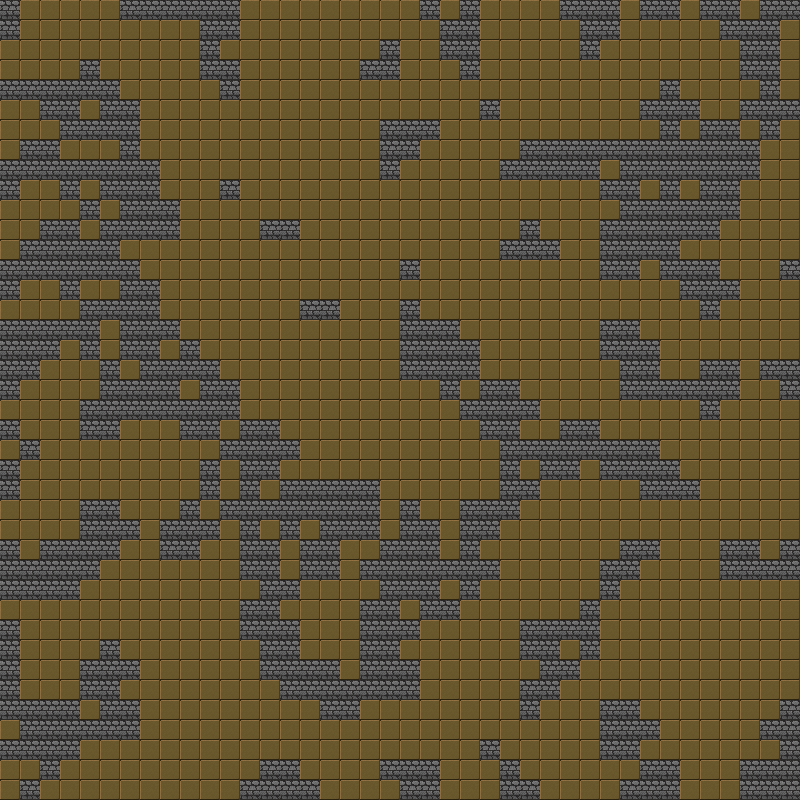
\includegraphics[width=\textwidth]{rouge/screenshot2}
		\caption{Step 2}
	\end{subfigure}	
	~
	\begin{subfigure}[b]{0.3\textwidth}
		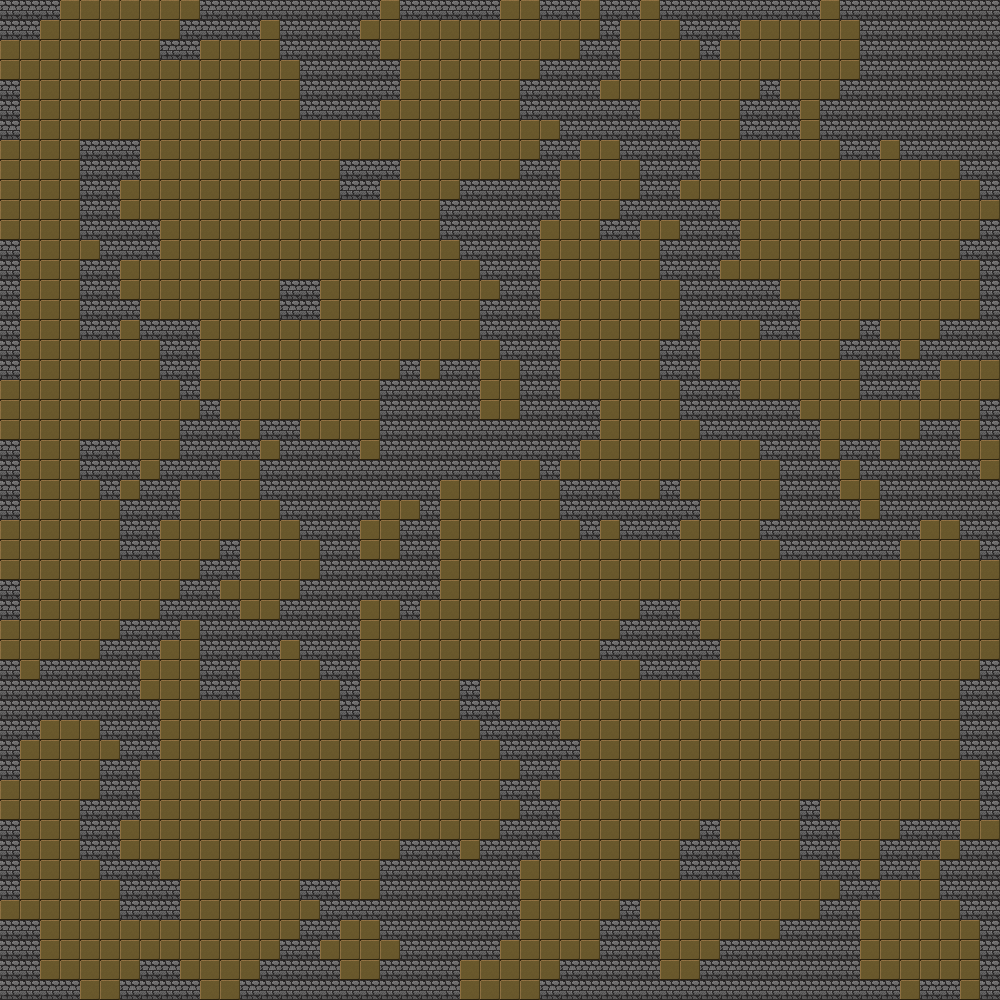
\includegraphics[width=\textwidth]{rouge/screenshot3}
		\caption{Step 3}
	\end{subfigure}		
	~
	\begin{subfigure}[b]{0.3\textwidth}
		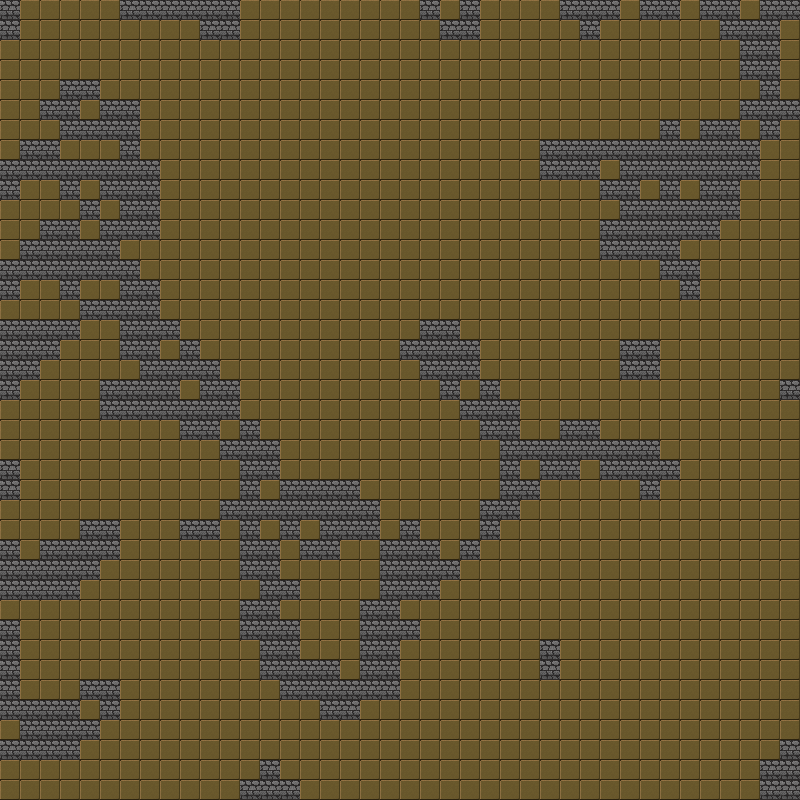
\includegraphics[width=\textwidth]{rouge/screenshot4}
		\caption{Step 4}
	\end{subfigure}
	~
	\begin{subfigure}[b]{0.3\textwidth}
		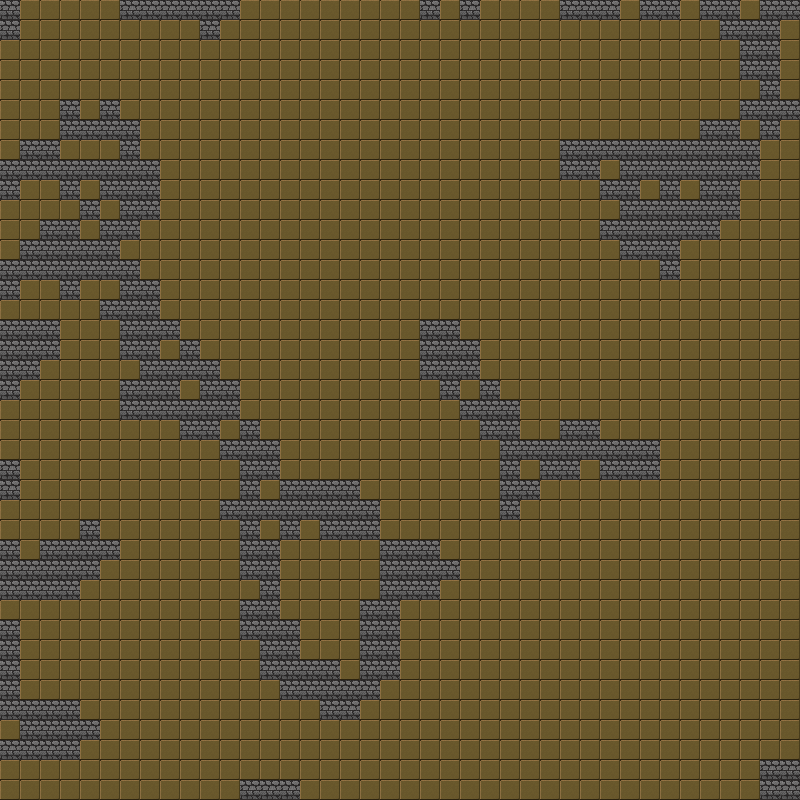
\includegraphics[width=\textwidth]{rouge/screenshot5}
		\caption{Step 5}
	\end{subfigure}	
	\caption{The generation of a 50 x 50 tilemap with 20 x 20 (pixels) tiles}\label{fig:rouge:screens}
\end{figure}

\section{Flood filling spaces}
As a recap, one of the \diage entities is the space. Spaces in \diage are representations of any game-world\footnote{hyphen?} space, be that the entire world, a city, a shop or a singular room. Spaces in Rouge are designated areas where the player can find shops and resolve \his objectives. These 'rooms' are generated using a simple tile-based flood-fill algorithm that circles round a selected tile. The algorithm has a maximum allowance that gets depleted by a tile's cost. This cost is higher for tiles that have fewer live neighbours than those that are encircled by them. This creates an the effect that corridors are more expensive to fill (thus have a lower grouping rate) and large open spaces are easy to fill all the way through.